\documentclass[conference,a4paper]{IEEEtran}

\usepackage{cite}
\usepackage{graphicx}

\newcommand{\blurb}[1]{\marginpar{{\tt !!!}}{\tt [... #1 ...]}}

\begin{document}

\title{A secondary screen architecture to accurately capture viewers' interactions in an iTV environment}

\author{\IEEEauthorblockN{Ricardo E. V. de S. Rosa}
\IEEEauthorblockA{Graduate Program in Electrical Engineering \\ Federal University of Minas Gerais \\ Av. Antônio Carlos 6627, 31270-901, \\Belo Horizonte, MG, Brazil\\
Email: ricardoerikson@ufmg.br}
\and
\IEEEauthorblockN{Lucas C. Cordeiro and Vicente F. de Lucena Junior}
\IEEEauthorblockA{Graduate Program in Electrical Engineering \\
Federal University of Amazonas \\
Manaus, AM, Brazil\\
Email: vicente@ufam.edu.br}
}
\maketitle

\begin{abstract}
TV watching is frequently seen as a social activity. People gather around the television for entertainment or information. Advances in TV technology have enabled the viewer to actively interact with the TV through interactive applications instead of just passively watching TV. Since the TV set is shared by many people and the interaction occurs by using a single remote control, it is difficult to accurately capture the individual needs from each viewer. It is also difficult to identify the context in which the interactions occur, e.g., to manage uniquely who is present in the environment and what is being watched on TV. In this paper, it is presented a novel architecture that facilitates viewers' individual interactions and contextual information in shared TV environments. One important application for this data consists of generating personalized content for single viewers and groups of viewers.
\end{abstract}

\IEEEpeerreviewmaketitle

\section{Introduction}

TV watching is essentially a social activity, where family, friends, or people with a common interest share the same space and TV set for entertainment or information. After many advances in technologies, for interactive and digital TV, it is possible to develop high-level applications to enrich the watching experience. Thus, the interaction between viewers and TV became more elaborated than simply change channels and adjust sound volume. In this scenario, the data generated by the interactions of millions of viewers can provide valuable information for content providers (CPs) to improve their services~\cite{Teixeira2010}.

The conventional remote control (RC) is typically used as the standard medium for viewers to interact with their TVs. However, this medium presents two notable problems: (1) to automatically identify the viewers who have possession of the RC; and (2) to capture contextualized viewers' interactions. As a result, the entire group of viewers (e.g., a family) is treated as a single viewer and the tastes that were inferred from the users in charge of the RC can be imposed on the tastes of the others.

Given the limitations of the conventional RC, a novel secondary screen architecture to identify viewers who are interacting with interactive TV (iTV) services is presented in this paper. Personal devices (e.g., smartphones and tablets) are used as secondary screens with the aim of capturing personal and contextualized interactions from each active viewer in iTV environments. By using proper machine learning algorithms, the personal data can reveal important information about viewers' tastes~\cite{Kim2012,Shin2009}. 

Since personal devices are almost ubiquitous, they stand out as a powerful mechanism to identify viewers by means of wireless communication technologies~\cite{Cabarcos2011}. In the architecture described in this paper, personal devices play an additional role as a medium of interaction since they are easy and intuitive to use in iTV environments, as pointed out in~\cite{Courtois2012}. An approach described in~\cite{Teixeira2010} has shown an architecture to capture viewers' interactions through a conventional RC. The architecture described in this paper goes further and captures individual and contextualized data. Since the TV environment is shared, the data about nearby viewers is captured to contextualize the interaction with the purpose of helping to infer the behaviors of one viewer toward others ones.

% In order to support millions of viewers, this architecture was implemented under a cloud computing based platform.

% Data about viewers' interactions are captured by personal devices (e.g., smartphones and tablets) that are used to mediate the interaction between viewers and the iTV device.

% \blurb{Achei que o inicio da introducao esta com muito bla bla bla. Tente ir direto ao ponto, dando uma visao geral da sua abordagem, as vantagens e desvantages com as outras abordagens existentes na literatura e as principais contribuicoes do seu trabalho. Por que voce acredita que os revisores devem aceitar o seu trabalho? Qual eh a inovacao? Quais sao as contribuicoes? Quais sao as diferencas para os trabalhos que ja existem. Diminua o bla bla bla do inicio e tente responder estas perguntas na introducao do seu trabalho.}

\section{Secondary Screen Architecture}

Initially, the CP infrastructure must provide an authentication mechanism so that viewers and their interactive TV (iTV) devices (e.g., set-top boxes or smart TVs) can be authenticated by the CP in order to use the secondary screen services. Once one iTV device is authenticated, the viewers in the TV environment must link their user accounts up with the iTV device. As a result, the viewer can use their personal device as a secondary screen, for that iTV device, in order to capture the viewers' interactions.

The architecture to accurately capture viewers interactions is shown in~\figurename~\ref{fig_architecture}. This architecture consists of secondary screen devices, which might be implemented in personal devices such as smartphones and tablets, an iTV device, and the CP infrastructure, which includes an application hosting infrastructure. Since applications in the TV domain have the potential to reach out millions of users at the same time, it is interesting that the CP infrastructure has the ability to deal with a large amount of incoming data~\cite{Lee2010}. The dashed green arrows represent the data flowing from the viewer to the CP infrastructure, while dotted blue arrows denote the flow from CP infrastructure to the viewers. The continuous black arrows represent the data flow inside the CP infrastructure.

\begin{figure}[!t]
	\centering
	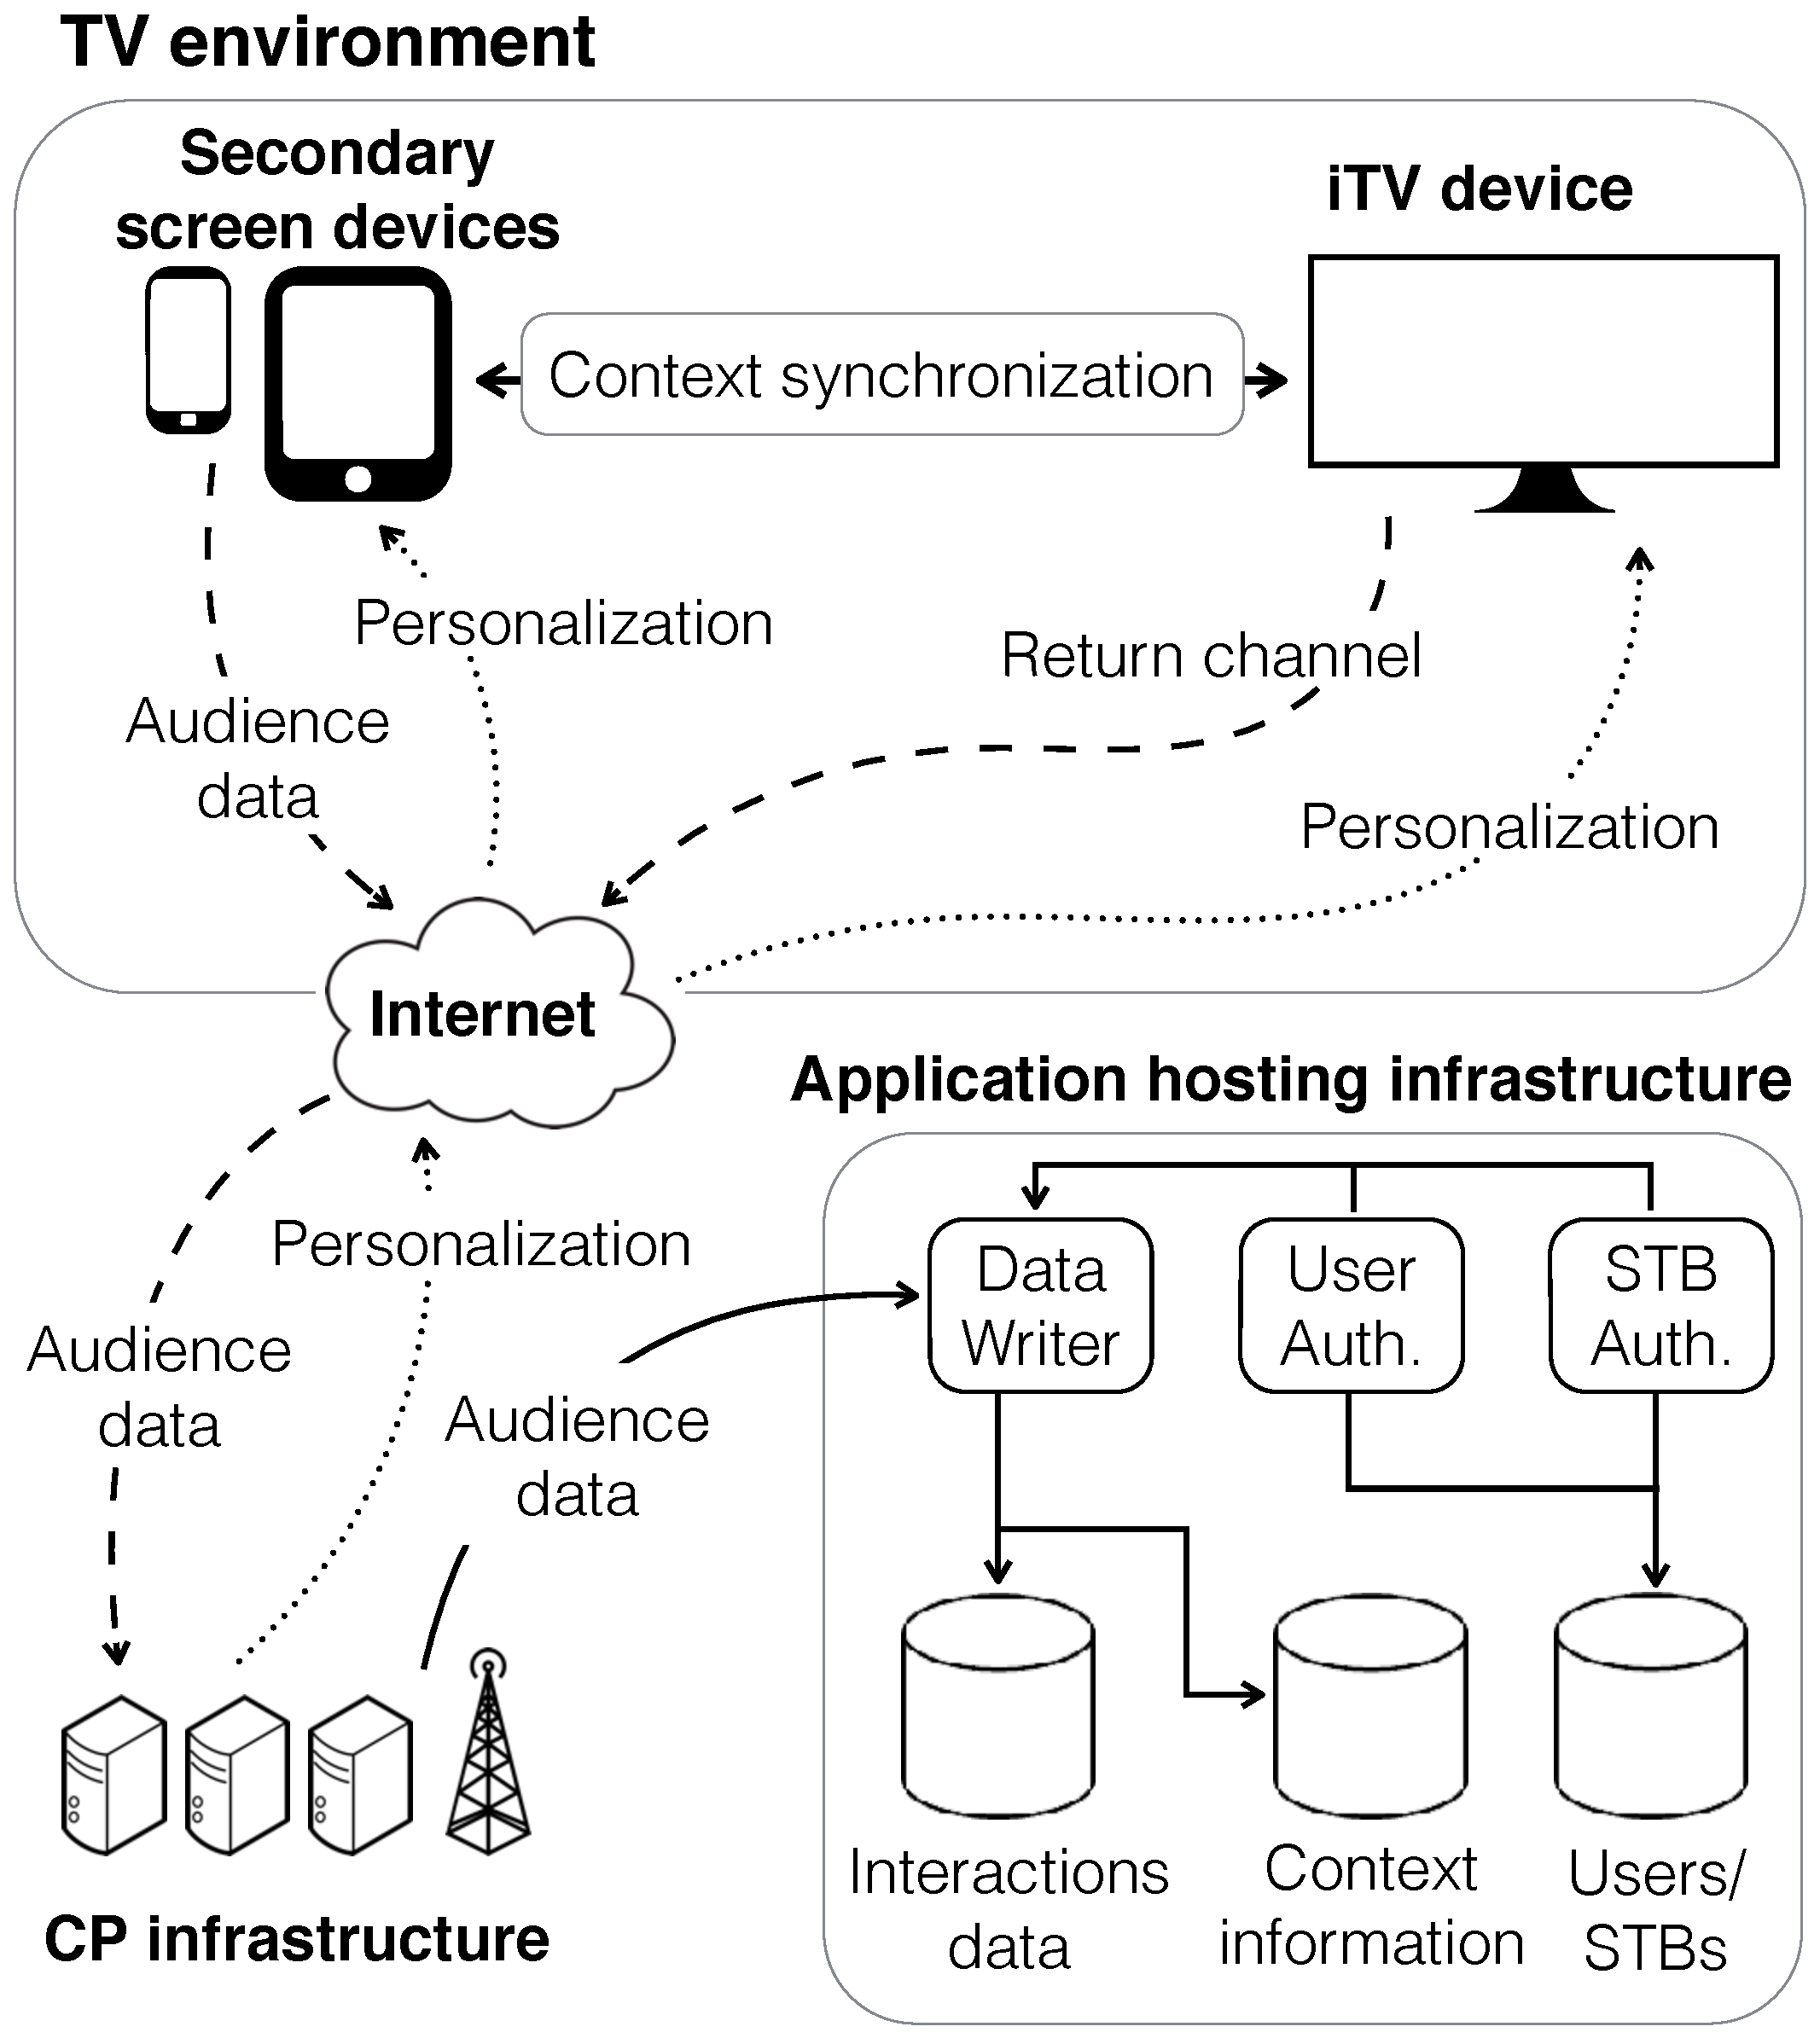
\includegraphics[width=3.5in]{img/architecture.pdf}
	\caption{Architecture to capture audience data. The viewers' interactions and the contextual information are captured and stored in the CP infrastructure.}
	\label{fig_architecture}
\end{figure}

A presence service detects physically nearby secondary screen devices that have the services necessary to establish a communication with an iTV device. Modern commercial operating systems for personal devices enable service discovery by using peer-to-peer or WiFi communication. This feature is particularly appropriate for the TV environment, once the secondary screen device must be wirelessly linked up with the iTV device. The devices are synchronized in order to update the contextual data about the viewer profile and the amount of people using a secondary device in the room. This contextual data can be used to learn how a viewer behaves towards other viewers. For example, a viewer behaves in a particular way while watching TV alone and the same viewer can behave in a different way while watching in group.

Viewers can use their secondary screen device to interact with TV by evaluating, commenting, sharing, or even recommending TV content to other viewers. The data related to those actions are naturally provided by the viewers, as part of the interaction, when using interactive applications (developed by the CP) installed in their secondary screen devices. The interactions and the contextual data are represented by the audience data, which is sent to CP infrastructure through Internet. Then, a Data Writer service stores the audience data related to each particular viewer and the iTV device.

The Data Writer components consists basically of web services that provide interoperability among secondary screen devices, iTV devices and the CP infrastructure. The main advantage of this approach is the independence of operating system and programming languages used in the personal devices.

Once the audience data is stored, the CP can use this data to derive valuable information about users' tastes. This information can be used to provide personalized content to viewers based on the current context. Thus, the personalized content can be delivered via Internet to the secondary screen device or even to the TV depending on the context.

% \blurb{Tens algum resumo dos resultados experimentais?}

\section{Conclusions}

The use of personal devices as secondary screens arises as a new trend in TV environments. This is paper presents an architecture to accurately capture audience data by using secondary screen devices and iTV devices. The implementation of this architecture is a work in progress, and take advantage of the ubiquity and interactive capabilities of secondary screen devices to identify viewers and provide feedback for CPs through viewers' interactions and contextual information. 

The captured data relates to a single viewer in a given context. By using proper machine learning algorithms, this data can provide valuable information about viewers. Knowing this information can be very useful for CPs to improve their services aiming to increase the audience and enrich user experience. As an example, CPs can deliver personalized content for a single person as well as for groups of people by using content recommendation algorithms.

An implementation of the architecture described in this paper was made using a commercial cloud computing environment, which plays the role of the CP infrastructure. A web application that consists of a content rating system was developed for both storing and retrieving viewers' tastes toward audio visual content provided by the CPs. Some RESTful web services were developed to store and retrieve viewers' interactions. The secondary screen applications were developed in Java and the viewer's interaction data were saved by means of HTTP requests.

The architecture described in this paper is also technically feasible to implement in Digital TV (DTV) systems and can be particularly interesting for CPs in DTV standards like the Brazilian (ISDB-TB) and the Japanese(ISDB-T). These standards support the use of mobile devices as part of the system. Since the mobile devices support the implementation of the DTV middleware, a cooperative exhibition of the DTV application can be managed with the iTV device, thus enabling the capture of viewers' interactions and contextual data.

\bibliographystyle{IEEEtran}
\bibliography{biblio}

\end{document}